% ====================================================================
%+
% SECTION:
%    cepheids.tex
%
% CHAPTER:
%    variables.tex
%
% ELEVATOR PITCH:
%
%-
% ====================================================================

\section{The Cepheid Mass-Luminosity Relation}
\def\secname{cepheids}\label{sec:\secname}

Classical Cepheids begin to pulsate once they evolve up the giant branch and
execute blueward loops on the HR diagram that take them into the Instability
Strip. Cepheid masses and luminosities in the instability strip are connected
through the Mass-Luminosity (ML) relation.  This ML relation is strongly
dependent on stellar evolution physics. Canonical/Non-canonical ML relations
arise from varying treatments of convective core overshoot and mass loss
\citep{1992A&A...258..397B,2000ApJ...529..293B,2013ApJ...768L...6M}.

Stellar pulsation models adopt a given ML relation and then compute a
theoretical light curve for a range of different temperatures and
metallicities. This theoretical light curve can then be transformed into LSST
wavebands using stellar atmospheres (\citep{Bono2000} and references therein) and
quantitatively compared to observed LSST light curves through Fourier
decomposition of the form
$$V = A_0 + \sum_{k=1}^{k=N}A_k cos(k\omega t + {\phi}_k),$$
where $\omega = 2\pi/P,$ with $P$ the period, $N$ is the order of the fit. The
coefficients $R_{k1}=A_k/A_1$ and ${\phi}_{k1}={\phi}_k - k{\phi}_1$ can be
computed for both theoretical and LSST observed light curves. These
coefficients are sensitive to the adopted $ML$ relation and other global
parameters such as metallicity and effective temperature.  By utilizing such a
decomposition, the multiwavelength light curves that the LSST will produce for
both Cepheids and RR Lyraes can rigorously constrain Cepheid and RR Lyrae
global stellar parameters such as the ML relation. Of course, knowledge of the
ML relation through this approach can then lead to another ``theoretical''
distance scale using both Cepheids and RR Lyraes.  However, in the case of
Cepheids, given good enough cadence in LSST bands and thus an accurate Fourier
decomposition with precisely known Fourier parameters, it will be possible to
discriminate between canonical and non-canonical ML relations and thus provide
constraints for stellar evolution physics. {\it A good Figure of Merit for
this science case would be one based on the precision with which
we can infer the parameters of these relations.}   

\citet{2014MNRAS.445.2655B} describes in detail the way the quantitative structure of
Cepheid and RR Lyrae light curves vary with period and optical band. Given
appropriate cadence, LSST light curves will provide accurate Fourier
decompositions at multiple wavelengths that can significantly augment these
results and provide an important database with which to connect quantitative
aspects of Cepheid and RR Lyrae light curve structure to pulsation envelope
physics. Two examples are the following.
\begin{itemize}
\item{1)} RRab stars found in stripe 82 of the
SDSS exhibit a flat Period-Color (PC) relation at minimum light at certain SDSS colors but not at others. LSST observations of RRab stars will be able
to augment this result and investigate if there are any links to the structural properties of observed light curves.
\item{2)} Short period ($\log P \le 0.4$) FU Cepheids in the SMC exhibit a noticeable break in their $(V-I)$ PC relation at certain phases of pulsation
phases. At the same period, the Fourier parameter $R_{21}$ displays a strong turnover. LSST data will be important in seeing if this result extends
to LSST colors.
\end{itemize}

\citet[and references therein]{2014MNRAS.445.2655B,2015MNRAS.447.3342B} have
demonstrated how Cepheid and RR Lyrae
Period-Color(PC)/Period-Luminosity (PL)/
Period-Wesenheit(PW)/Period-Luminosity-Color(PLC) relations vary significantly
both as a function pulsation phase and period and observation band.  The LSST
database on Cepheids and RR Lyraes will provide an excellent database to further
investigate the variation of these relations with pulsation phase with a view
to understanding pulsation physics and constraining theoeretical models.
Currently, the literature only discusses these relations at mean light, that
is the average over pulsation phase. Yet this averaging process masks
some dependencies: there are pulsation phases with very high/low PL/PC
dispersion and there are some phases where the relation is highly nonlinear.
In the era of precision cosmology, it is important to understand the tools that
we use to construct a distance scale. The LSST database on Cepheids and RR
Lyraes will be an important database with which to investigate the multiphase
properties of PL/PC/PW/PLC relations.

What cadence is required for ``accurate multiwavelength Fourier
decomposition''? Cepheids and RR Lyraes are strictly periodic. Then for known variables, whose periods are already known, such
Fourier decompositions can be carried out on folded light curves. In such
situations given a cadence, one possible measure of the success of this Fourier
decomposition could be the maximum phase gap in the folded light curve. Another
measure could be the error on the Fourier parameters
\citep{1986A&A...170...59P}. One way forward is to carry out a detailed
Fourier analysis of any one simulated schedule.

\subsection{Description of Relevant Metrics}
\label{sec:\chpname:variablemetrics}

Despite the range in scientific motivation for the cases presented
in this chapter,
there are some common metrics that are widely applicable (or may
be combined in a variety of ways with other metrics to suit a variety of
applications).
\new{The present science case provides as good a venue as
any in which to introduce these common metrics.}

%\subsection{Metrics}
%\label{sec:\chpname:metrics}

\begin{center}
\begin{tabular}{| p{5cm} |p{10cm} |}
\hline Metric & Description\\
\hline
Eclipsing/transiting system discovery & Fraction of discoveries vs fractional duration of eclipse\\
Lightcurve shape recovery & ... \\
%Transiting exoplanets (depth dependent) & Fraction of discoveries vs fractional duration of eclipse\\
Phase gap & Histogram vs period of the median and maximum phase gaps achieved in all fields\\
Period determination (period dependent) & Fraction of targets vs survey duration, for which the period can be determined to 5-sigma confidence\\
Period variability (period dependent) & Fraction of targets vs survey duration, for which a period change of 1\% can be determined with 5-sigma confidence\\
  \hline \end{tabular}
 \end{center}

The ability to identify that an object is periodic, and to correctly
determine that object's period, are widely applicable measures of
discovery. In the case of regular variables (as outlined below), these
two measures together can uniquely identify a population. Other kinds of
periodic systems (transiting planets for example) also require a
measurement of periodicity, but have a much wider range of relevant
periods, and looser requirements on the strictness of that periodicity.

\citet{LundEtal2016} discuss three {\it diagnostic} metrics that have been
incorporated into the MAF. Two of these metrics deal explicitly with time
variable behavior: a) observational triplets, and b) detection of periodic
variability.

%%%%%%%%%%%%%%%%%%%%%%%%%%%%%%%%%
\begin{figure}[tbh!]
%\vskip -4.1in
%\hskip -0.5in
%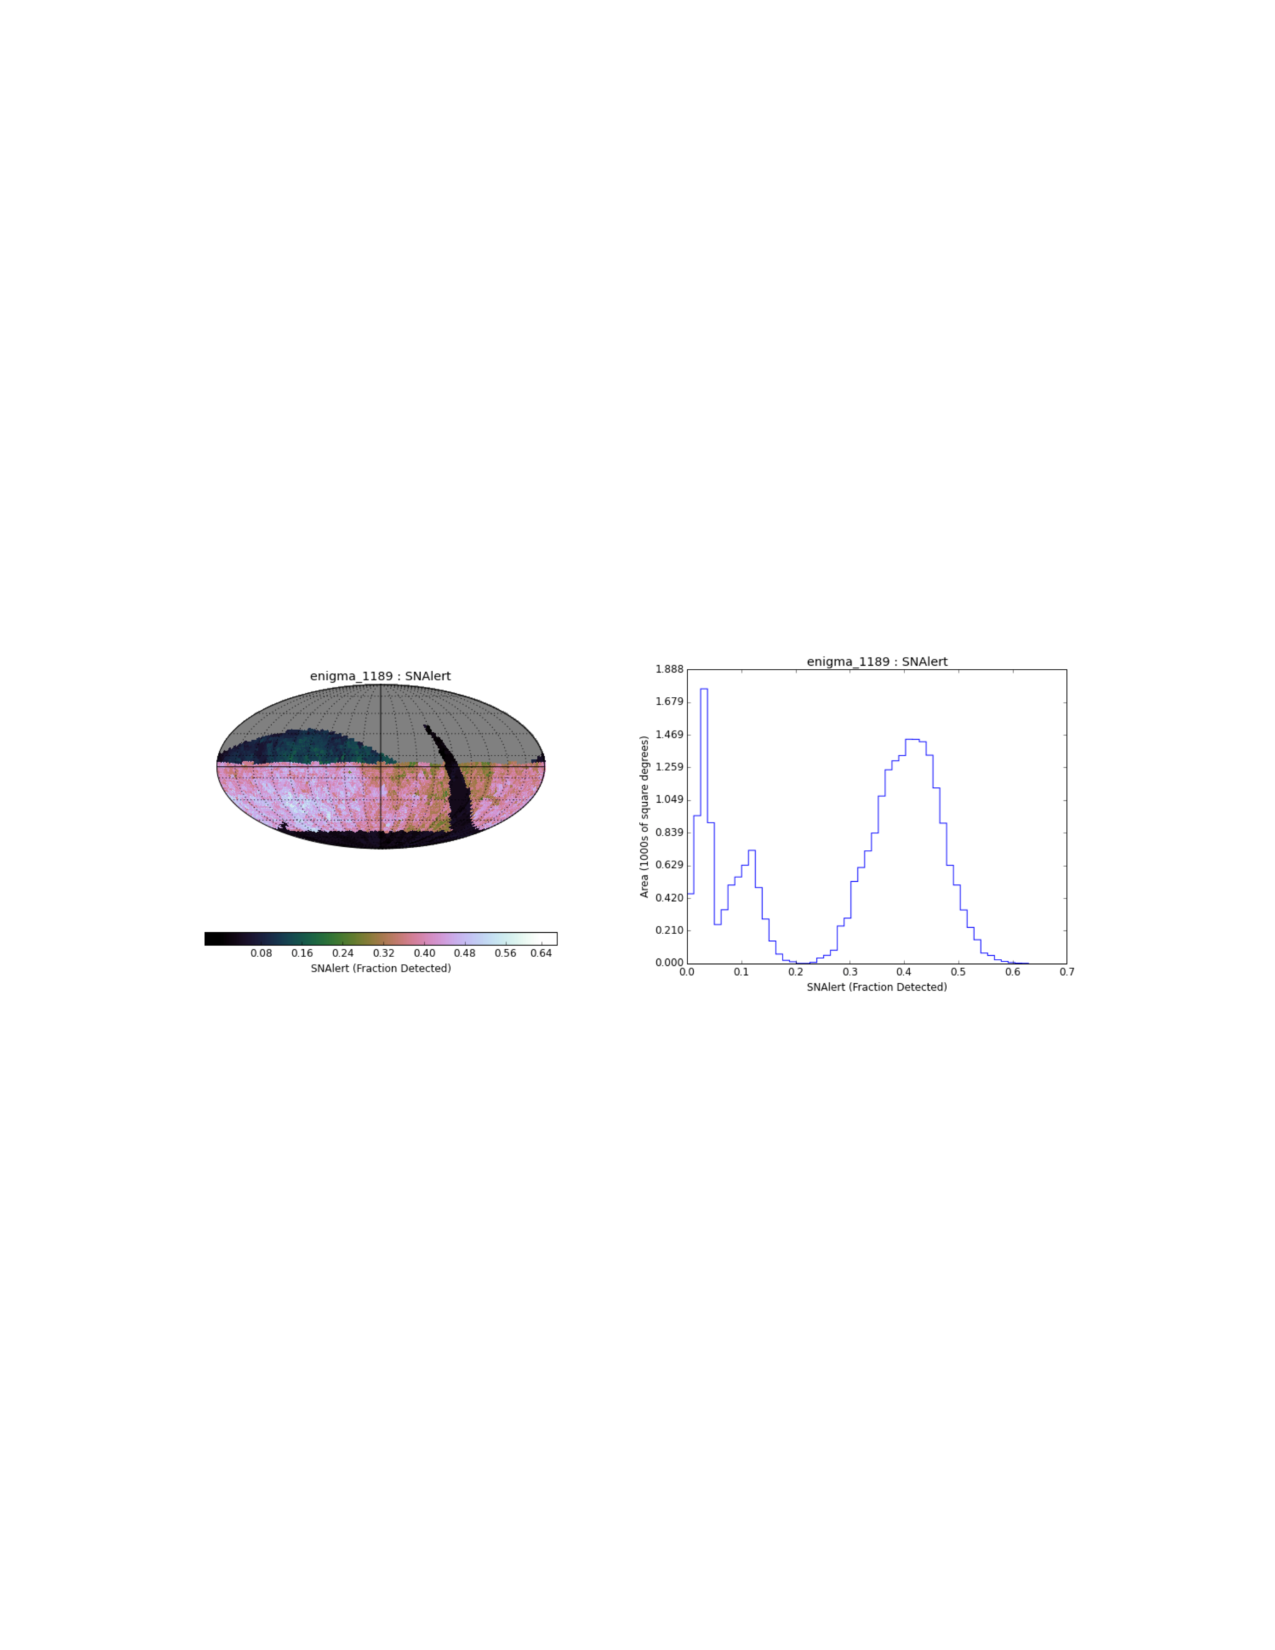
\includegraphics[angle=0,width=1.19\hsize:,clip]{figs/enigma1189_earlySNe.pdf}
%\vskip -4.0in
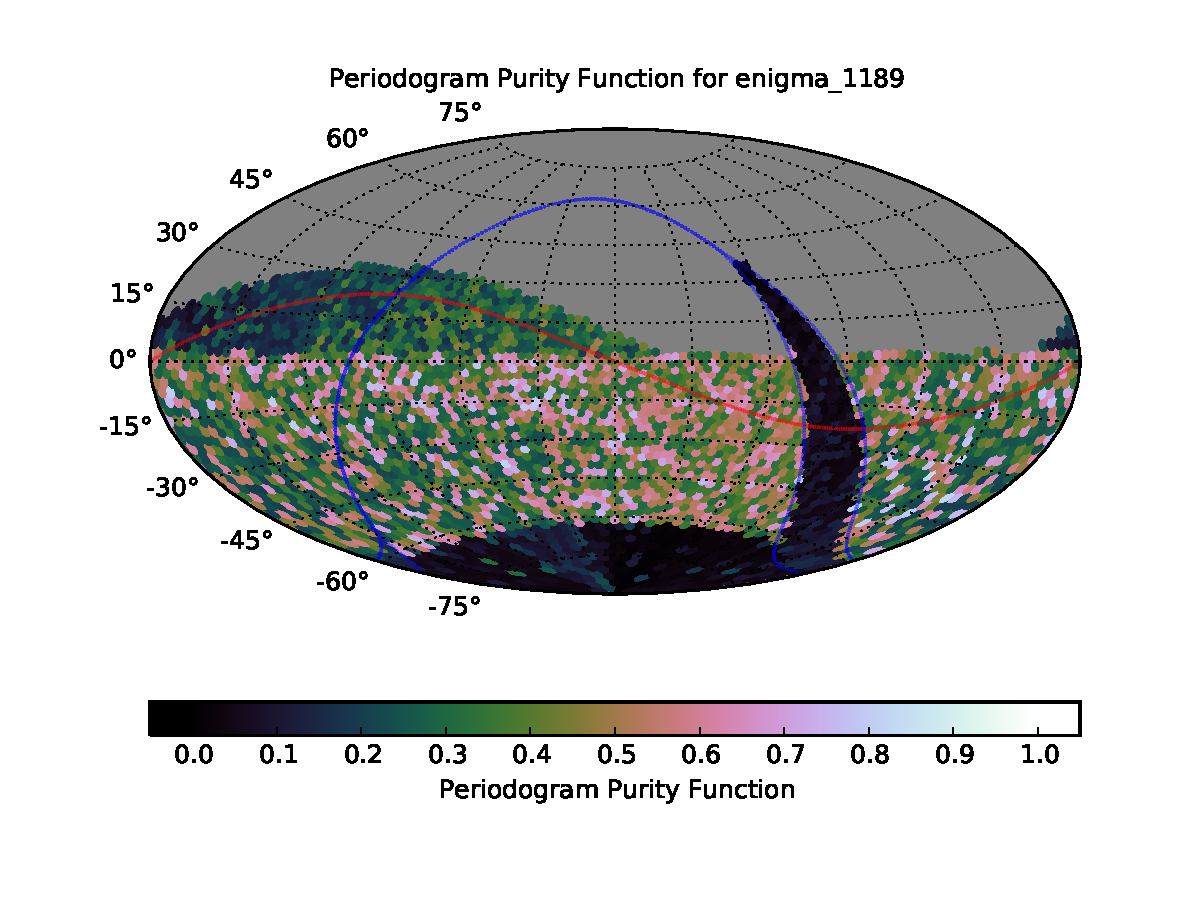
\includegraphics{figs/variables/enigma_1189_PeriodogramPurity_OPSI_SkyMap.pdf}
\caption{The value for the Periodogram Purity Function for candidate
Baseline Cadence \opsimdbref{db:baseCadence}. The Periodogram Purity
Function provides a measure of the power lost due to aliasing.}
\label{fig:enigmaPeriodogramPurity}
\end{figure}
%%%%%%%%%%%%%%%%%%%%%%%%%%%%%%%%%


%%%%%%%%%%%%%%%%%%%%%%%%%%%%%%%%%
\begin{figure}[tbh!]
%\vskip -4.1in
%\hskip -0.5in
%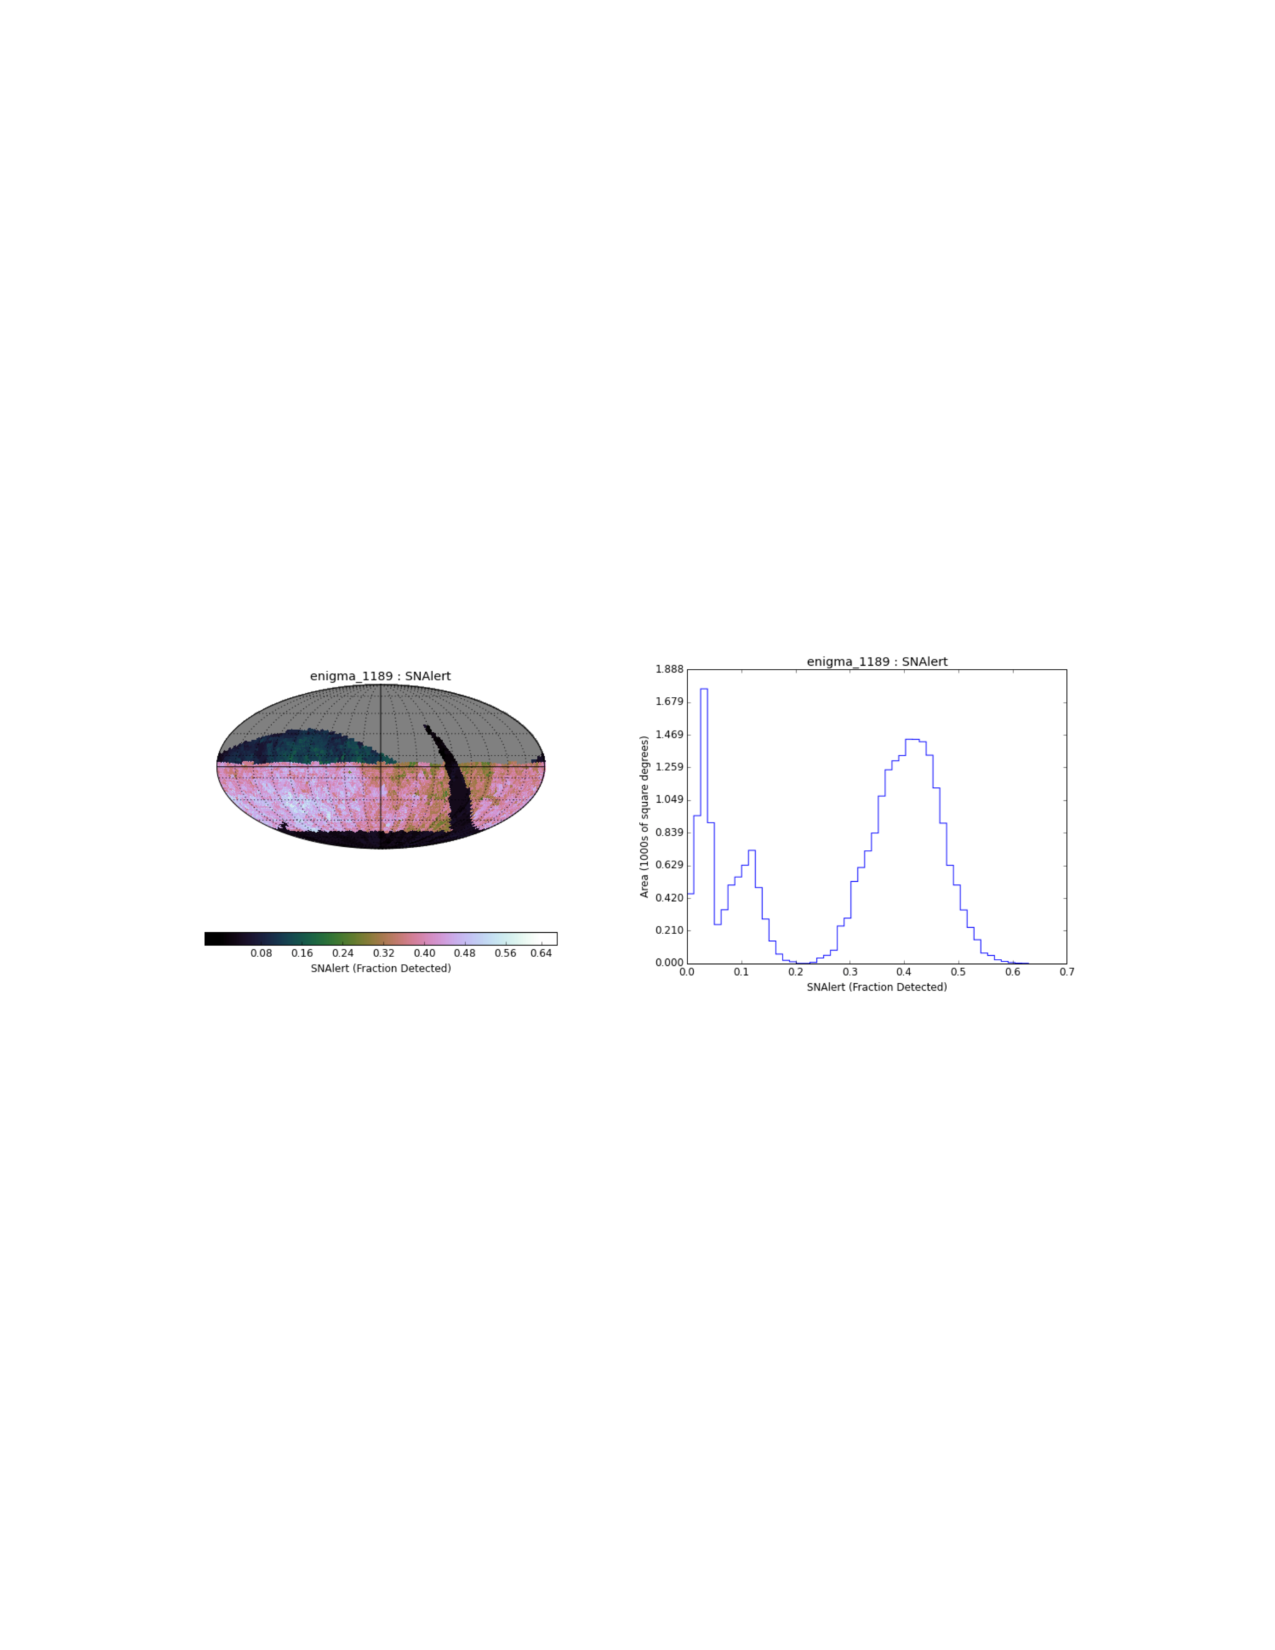
\includegraphics[angle=0,width=1.19\hsize:,clip]{figs/enigma1189_earlySNe.pdf}
%\vskip -4.0in
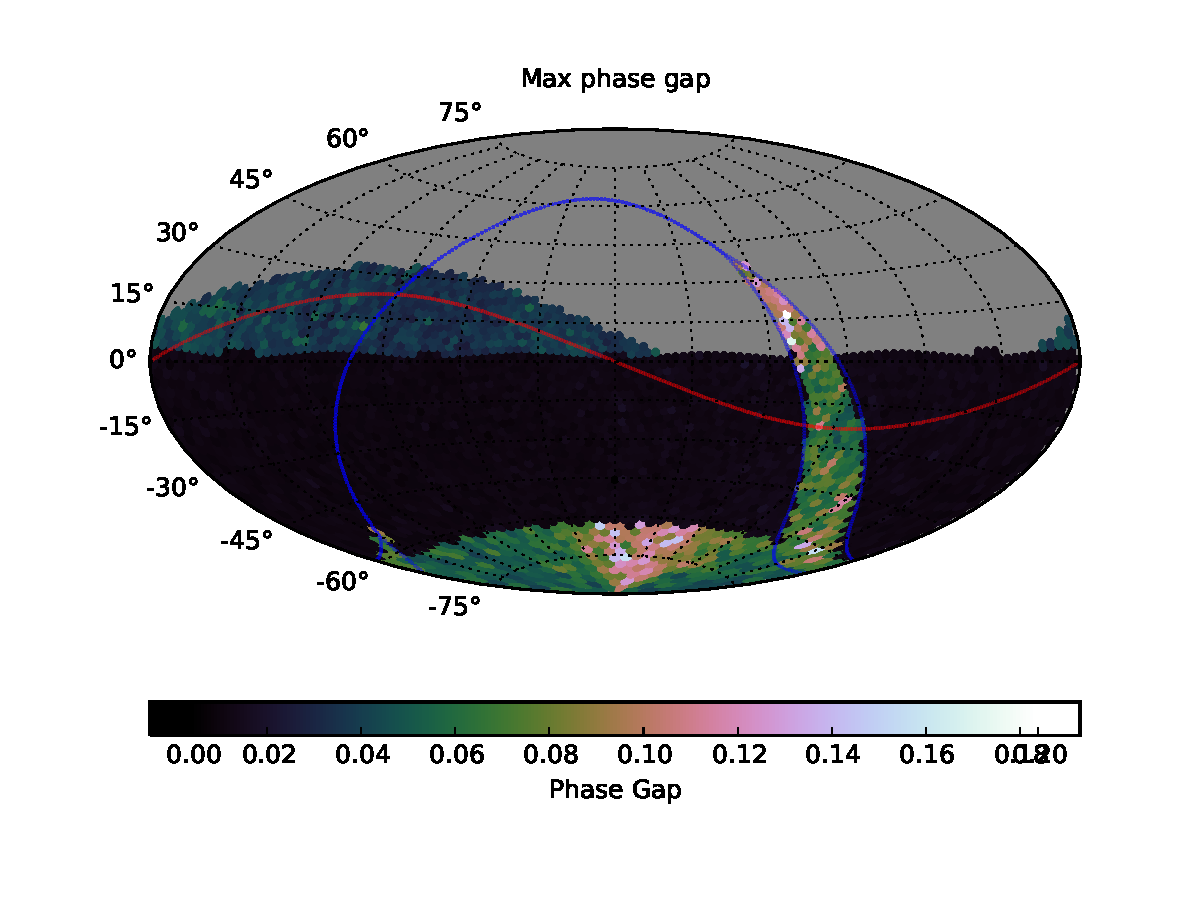
\includegraphics{figs/variables/enigma_1189_Phase_Gap_MedianGap_OPSI_SkyMap.pdf}
\caption{The median phase gap for candidate Baseline Cadence \opsimdbref{db:baseCadence}.
The PhaseGapMetric looks at periods between 3 and 35 days by default.}
\label{fig:enigmaMedianGap}
\end{figure}
%%%%%%%%%%%%%%%%%%%%%%%%%%%%%%%%%

%%%%%%%%%%%%%%%%%%%%%%%%%%%%%%%%%
\begin{figure}[tbh!]
%\vskip -4.1in
%\hskip -0.5in
%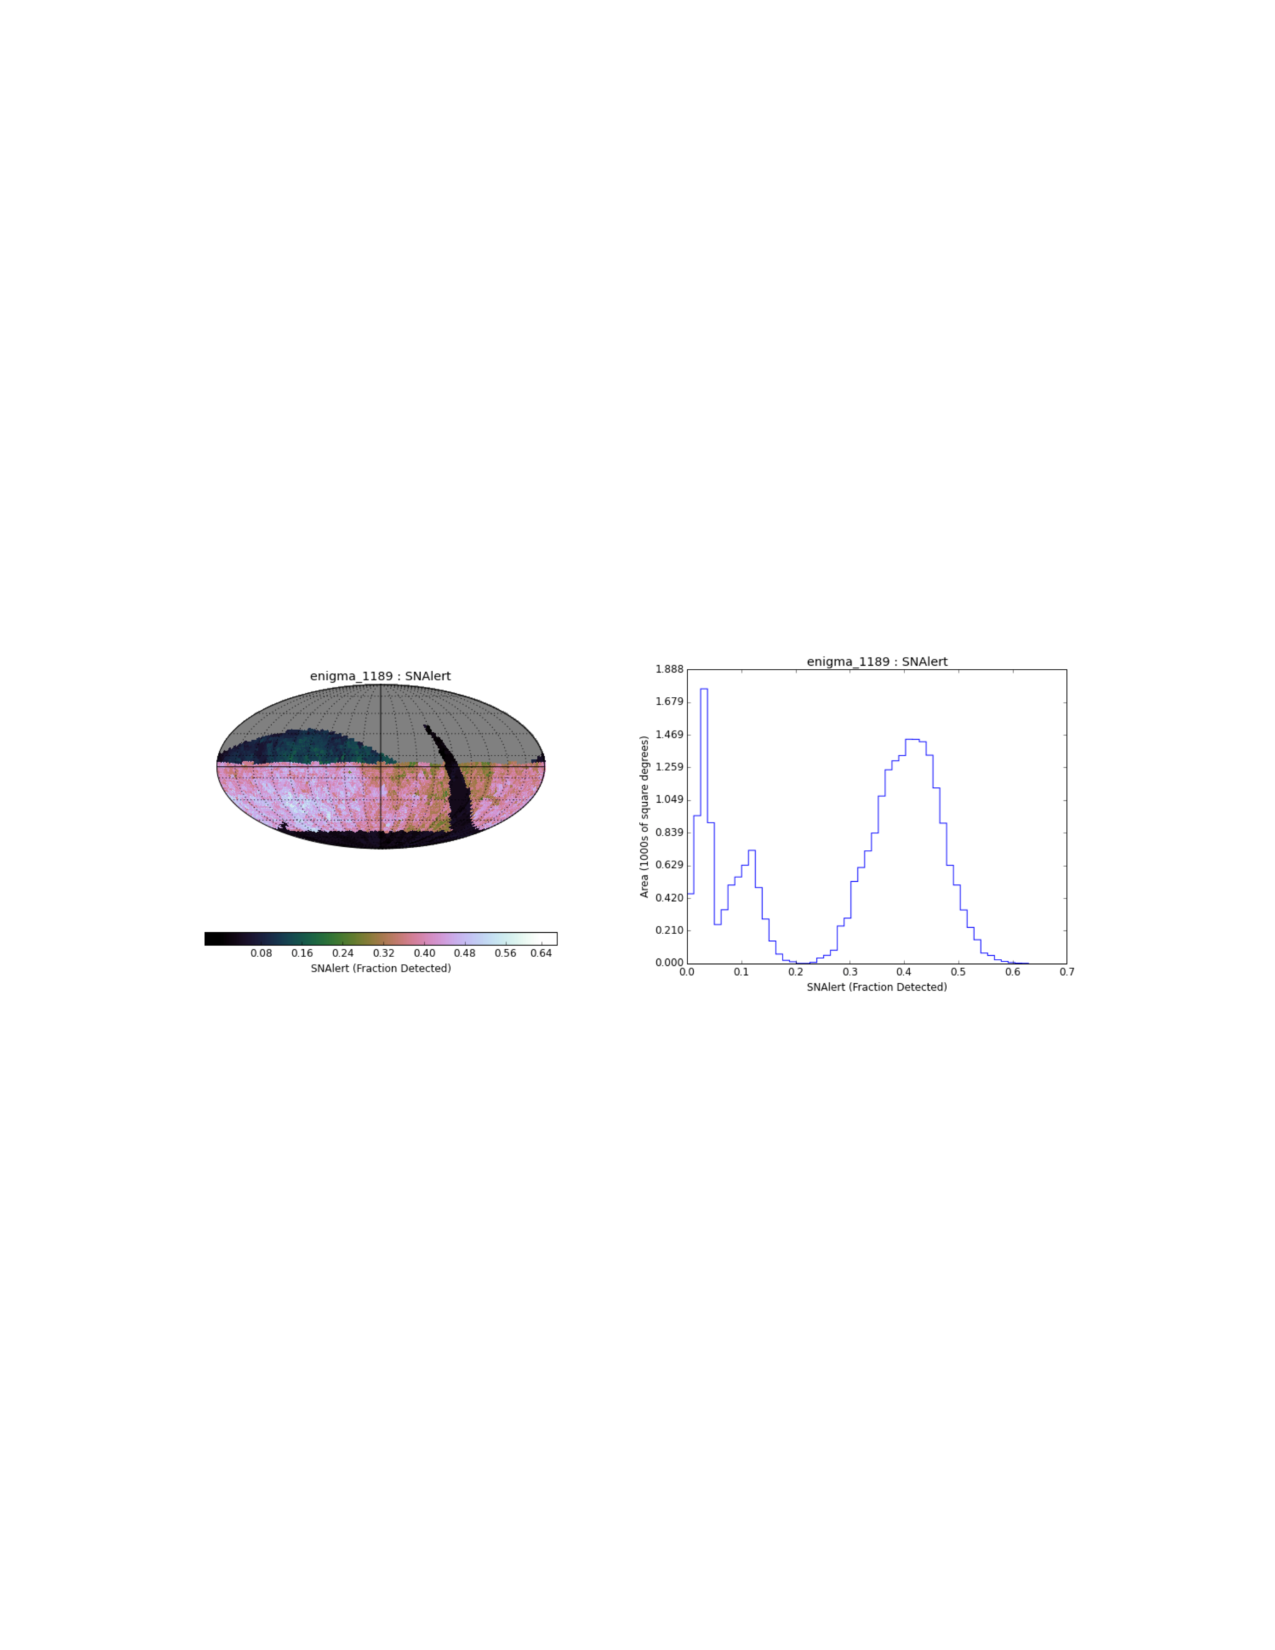
\includegraphics[angle=0,width=1.19\hsize:,clip]{figs/enigma1189_earlySNe.pdf}
%\vskip -4.0in
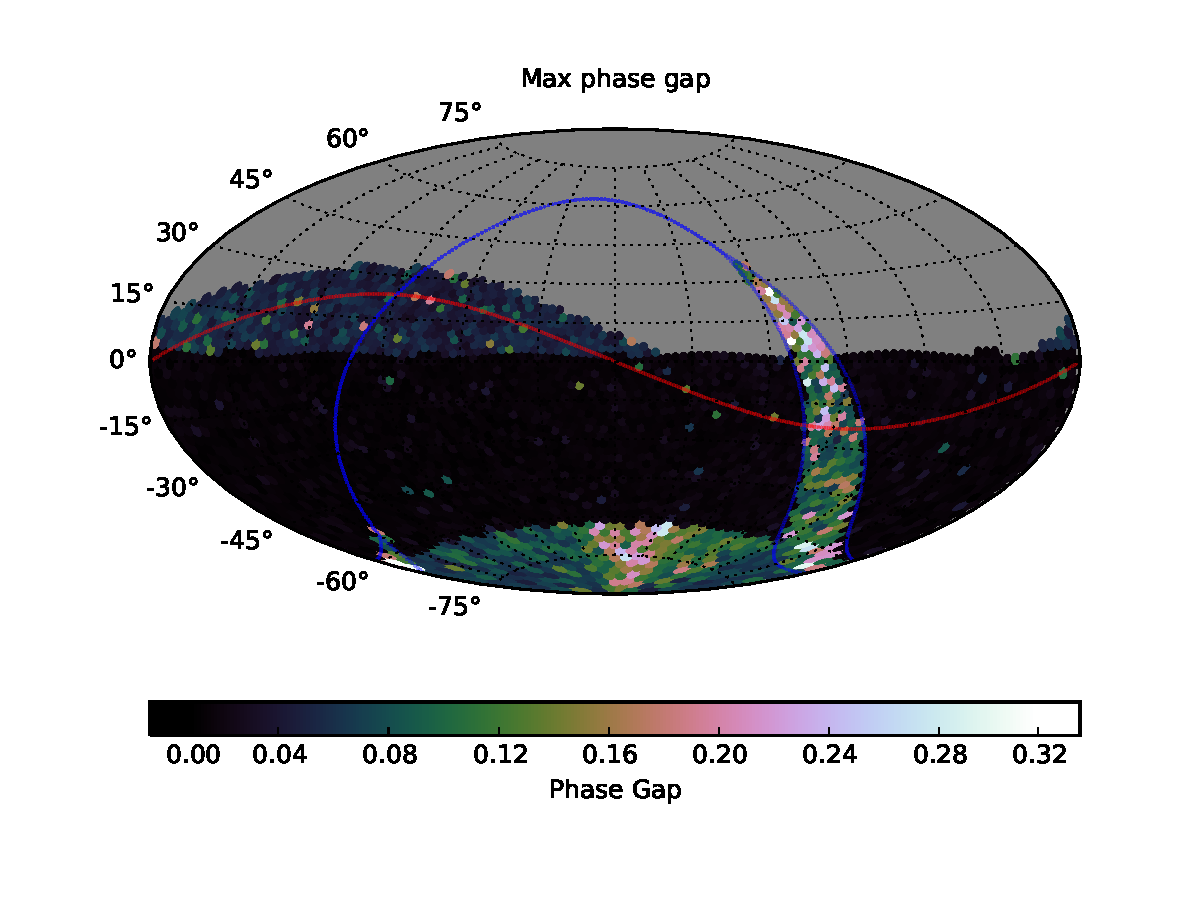
\includegraphics{figs/variables/enigma_1189_Phase_Gap_LargestGap_OPSI_SkyMap.pdf}
\caption{The maximum phase gap for candidate Baseline Cadence \opsimdbref{db:baseCadence}.
The PhaseGapMetric looks at periods between 3 and 35 days by default.}
\label{fig:enigmaMaxGap}
\end{figure}
%%%%%%%%%%%%%%%%%%%%%%%%%%%%%%%%%

\subsubsection{Periodogram purity function (PeriodicMetric)}

This metric calculates the Fourier power spectral window function of each field
\citep{1987AJ.....93..968R} as a means of quantifying the completeness of phase
coverage for a given periodic variable. The periodogram purity is defined as 1
minus the Fourier power spectral window function. in the perfect case, all
power in the window function is concentrated in a delta function at zero, and
is zero at all other frequencies. As power ``leaks'' away from the correct
frequency as a consequence of discrete, non-ideal data sampling, the
periodogram becomes more structured. For the purposes of MAF metrics, which are
designed to quantify performance as a single number, the periodogram purity is
quantified as the minimum value of the periodogram purity function at non-zero
frequency shifts; the ideal case would be a periodogram purity metric value of
1.

\subsubsection{Phase Gap Metric (PhaseGapMetric)}

The Phase Gap Metric is designed to examine the largest phase gaps in
the observing schedule. For a given point in the sky, a series of
periods are randomly selected (by default, 5 periods), with a default
minimum of 3 days and maximum of 35 days. The largest phase gap for each
period is calculated, and the metric plots the median
(\autoref{fig:enigmaMedianGap}) and maximum (\autoref{fig:enigmaMaxGap})
of this subset of values that contains the maximum phase gap per period.
The Phase Gap Metric is part of varMetrics.

\subsubsection{Period Deviation Metric (PeriodDeviationMetric)}

The Period Deviation Metric calculates the error in recovering the
correct period of a sinusoid using a given observing schedule and a
Lomb-Scargle periodogram. For a given point in the sky, a series of
periods are randomly selected (by default, 5 periods), and the metric
returns the worst period deviation, and the period at which this
occurred. The Period Deviation Metric is part of varMetrics.

%\subsection{Proposed Metrics}

%The following is a raw list of metric ideas; these need specificity and further description.

%FWHM of the window function (to quantify sampling)

%Maximum hour angle difference

%Fraction of discoveries vs fractional duration of eclipse

%Fraction of targets vs survey duration, for which the period can be determined to 5-sigma confidence

%Fraction of targets vs survey duration, for which a period change of 1$\%$ can be determined with 5-sigma confidence
